\documentclass[12pt]{letter}
\usepackage{amsmath,amsfonts,amsthm,amstext,amssymb,graphicx, multicol,fancyhdr,lastpage,fullpage,framed,fancybox,enumerate,tikz,color,mathrsfs, polynom, pifont, stmaryrd}
\usepackage[margin=0.5in,headsep=3pt, headheight=15pt]{geometry}

% ----------------------------------------------------------
% Custom Definitions, Commands, Environments, etc.

% Sets of numbers
\def\R{\mathbb{R}} % The reals
\def\N{\mathbb{N}} % The naturals
\def\Z{\mathbb{Z}} % The integers
\def\Q{\mathbb{Q}} % The rationals
\def\C{\mathbb{C}} % The complex
\def\F{\mathbb{F}} % Field

% Blank space\\
\newcommand{\blank}[1]{\underline{\hspace{#1}}} % Blank space

% Change font colors
\newcommand{\cyan}[1]{{\color{cyan}{#1}}} % Changes font to cyan
\newcommand{\red}[1]{{\color{red}{#1}}} % Changes font to red
\newcommand{\magenta}[1]{{\color{magenta}{#1}}} % Changes font to magenta
\newcommand{\orange}[1]{{\color{orange}{#1}}} % Changes font to orange
\newcommand{\yellow}[1]{{\color{yellow}{#1}}} % Changes font to yellow
\newcommand{\violet}[1]{{\color{violet}{#1}}} % Changes font to violet
\newcommand{\green}[1]{{\color{green}{#1}}} % Changes font to green
\newcommand{\blue}[1]{{\color{blue}{#1}}} % Changes font to blue
\newcommand{\white}[1]{{\color{white}{#1}}} % Changes font to white

% Fitted inclusion symbols
\newcommand{\fp}[1]{\left({#1}\right)} % Fitted parentheses around content
\newcommand{\fb}[1]{\left[{#1}\right]} % Fitted brackets
\newcommand{\lhoi}[1]{\left({#1}\right]} % Left half-open interval
\newcommand{\rhoi}[1]{\left[{#1}\right)} % Right half-open interval
\newcommand{\set}[1]{\left\{{#1}\right\}} % Fitted braces (useful for sets)
\newcommand{\av}[1]{\left|{#1}\right|} % Fitted absolute value bars
\newcommand{\step}[1]{\left\llbracket {#1} \right\rrbracket}

% Augmented Matrix Environment
\newenvironment{amatrix}[1]{%
	\left[\begin{array}{@{}*{#1}{c}|c@{}}
	}{%
	\end{array}\right]
}

% Miscellaneous
\def\then{\Rightarrow}
\def\to{\rightarrow}
\def\d{^{\circ}}
\newcommand{\?}{\stackrel{?}{=}}
\newcommand{\cmark}{\text{ \ding{51}}}
\newcommand{\xmark}{\text{ \ding{55}}}



% Coordinate Plane (Four-Quadrant)
\def\coordplane {
	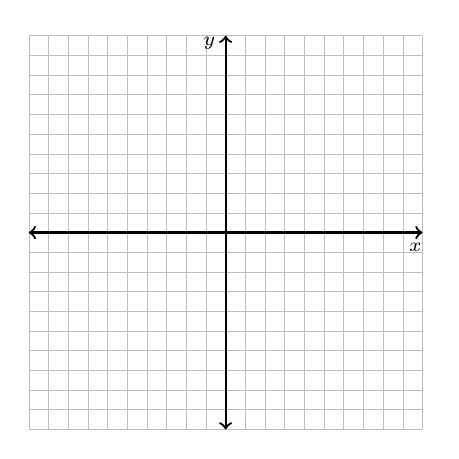
\begin{tikzpicture}        \draw[step=0.25cm,black,very thin,opacity=0.25] (-2.5cm, -2.5cm) grid (2.5cm, 2.5cm);
		\draw[<->,thick,black] (-2.5cm, 0) -- (2.5cm, 0) node[anchor=north west,pos=0.94,font=\scriptsize]{$x$};
		\draw[<->,thick,black] (0,-2.5cm) -- (0, 2.5cm) node[anchor=south east,font=\scriptsize,pos=0.94]{$y$};
	\end{tikzpicture}
}

% Coordinate Plane (One-Quadrant)
\def\onequad {
	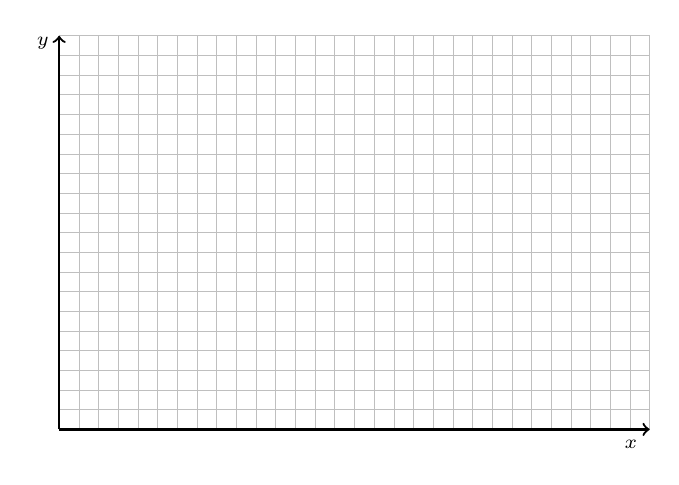
\begin{tikzpicture}
		\draw[step=0.25cm, black, very thin, opacity=0.25] (0,0) grid (7.5cm,5cm);
		\draw[->, thick, black] (0,0) -- (7.5cm, 0) node[anchor=north west,font=\scriptsize,pos=0.94]{$x$};
		\draw[->, black, thick] (0,0) -- (0,5cm) node[anchor=south east,font=\scriptsize,pos=0.94]{$y$};
	\end{tikzpicture}
}

% Counters
\newcounter{exercise}

% Exercise environment (auto-numbered)
\newenvironment{exercise}[1][]{\begin{framed}\refstepcounter{exercise}\textbf{Exercise~\theexercise:} #1}{\end{framed}}

% Book exercise environment
\newenvironment{bex}[2] {
	\begin{framed}
		\textbf{Book Exercise {#1}:} #2
	\end{framed}	
}
% ----------------------------------------------------------

% ----------------------------------------------------------
% Header and Footer Information
% \pagestyle{fancy}
% \fancyhf{}
% \renewcommand{\headrulewidth}{0pt}
% \rhead{Name: \blank{2in}}
% \lhead{@}
% \rfoot{Page \thepage \, of \,\pageref{LastPage}}
% ----------------------------------------------------------
\author{Jacob Ayers}

\begin{document}
	
	\begin{center}
		\textbf{MAT 130 Weekly Schedule \\ Fall \red{Year}}
	\end{center}
	\textbf{Live Conferences:} Every \red{day} at \red{time} (required Week 1; optional afterward)
	
	\textbf{Week 1} \begin{itemize} \vspace{-12pt}
		\item Thursday: First Week Attendance Assignment due @ 2:00
		\item Video Lesson \#1 (P.1 and P.2)
		\item Video Lesson \#2 (P.3 and P.4)
	\end{itemize}

	\textbf{Week 2} \begin{itemize} \vspace{-12pt}
		\item Wednesday: Assignment 1 due @ 11:59 pm
		\item Video Lesson \#3 (P.5 and P.6)
		\item Video Lesson \#4 (1.1 and 1.2)
	\end{itemize}

	\textbf{Week 3} \begin{itemize} \vspace{-12pt}
		\item Wednesday: Assignment 2 due @ 11:59 pm
		\item Video Lesson \#5 (1.3 and 1.4)
		\item Video Lesson \#6 (1.5 and 1.6)
	\end{itemize}

	\textbf{Week 4} \begin{itemize} \vspace{-12pt}
		\item Wednesday: Assignment 3 due @ 11:59 pm
		\item Video Lesson \#7 (1.7 and 1.8)
		\item Video Lesson \#8 (2.1 and 2.2)
	\end{itemize}

	\textbf{Week 5} \begin{itemize} \vspace{-12pt}
		\item Wednesday: Assignment 4 due @ 11:59 pm
		\item Video Lesson \#9 (2.3-2.5)
		\item Video Lesson \#10 (2.6 and 2.7)
	\end{itemize}

	\textbf{Week 6} \begin{itemize} \vspace{-12pt}
		\item Wednesday: Assignment 5 due @ 11:59 pm
		\item Exam 1 Study Guide posted to Moodle (optional, but highly recommended)
	\end{itemize}

	\textbf{Week 7} \begin{itemize} \vspace{-12pt}
		\item Wednesday: Exam 1 (Chapters P-2)
		\item Video Lesson \#11 (3.1 and 3.2)
		\item Video Lesson \#12 (3.3)
	\end{itemize}

	\textbf{Week 8} \begin{itemize} \vspace{-12pt}
		\item Wednesday: Assignment 6 due @ 11:59 pm
		\item Video Lesson \#13 (3.4)
		\item Video Lesson \#14 (3.5)
		\item Video Lesson \#15 (4.1)
	\end{itemize}

	\textbf{Week 9} \begin{itemize}
		\item Wednesday: Assignment 7 due @ 11:59 pm
		\item Video Lesson \#16 (4.2)
		\item Video Lesson \#17 (5.1)
	\end{itemize}

	\textbf{Week 10} \begin{itemize} \vspace{-12pt}
		\item Wednesday: Assignment 8 due @ 11:59 pm
		\item Video Lesson \#18 (5.2)
		\item Video Lesson \#19 (5.3)
	\end{itemize}

	\textbf{Week 11} \begin{itemize} \vspace{-12pt}
		\item Wednesday: Assignment 9 due @ 11:59 pm
		\item Video Lesson \#20 (5.4)
		\item Video Lesson \#21 (5.5)
	\end{itemize}

	\textbf{Week 12} \begin{itemize} \vspace{-12pt}
		\item Wednesday: Assignment 10 due @ 11:59 pm
		\item Exam 2 Study Guide posted to Moodle (optional, but highly recommended)
	\end{itemize}

	\textbf{Week 13} \begin{itemize} \vspace{-12pt}
		\item Wednesday: Exam 2 (Chapters 3-5)
		\item Video Lesson \#22 (9.1 and 9.2)
		\item Video Lesson \#23 (9.3)
	\end{itemize}

	\textbf{Week 14} \begin{itemize} \vspace{-12pt}
		\item Wednesday: Assignment 11 due @ 11:59 pm
		\item Video Lesson \#24 (10.1)
		\item Video Lesson \#25 (10.1)
	\end{itemize}

	\textbf{Week 15} \begin{itemize} \vspace{-12pt}
		\item Thanksgiving - No Course Responsibilities
	\end{itemize}

	\textbf{Week 16} \begin{itemize} \vspace{-12pt}
		\item Wednesday: Assignment 12 due @ 11:59 pm
		\item Video Lesson \#26 (10.2)
		\item Video Lesson \#27 (10.4)
		\item Final Exam Study Guide posted to Moodle (optional, but highly recommended)
	\end{itemize}

	\textbf{Week 17} \begin{itemize} \vspace{-12pt}
		\item Thursday: Final Exam due at 11:59 pm
	\end{itemize}

\end{document}